\chapter{Introduction}
\label{ch:introduction}

\section{Overview and Background of the Study}
There have been many advancements in environmental monitoring in the last ten years, mostly due to the proliferation of Internet of Things (IoT) technology. The conventional approach involved using very few specialized and expensive stations, which provided poor spatial resolution and were tough to deploy in remote and hazardous locations. On the other hand, modern IoT-based systems use dense low-power and low-cost sensors to gather detailed information on a geographical basis. These systems have proven to be essential in different areas such as smart agriculture, urban climate sensing, disaster management, and public health.

The rise of digitization in the physical world has increased the amount of data produced from sensor networks to exponential proportions. Real-time capturing of environmental parameters such as temperature, humidity, air quality, and air pressure enables quick decision-making and accurate prediction modeling. Nonetheless, the trend towards pervasive sensing brings about several infrastructure problems. The use of devices such as the Raspberry Pi and the ESP8266 as edge devices is commonplace since they are inexpensive and flexible; however, they function under tight limitations of energy availability, computing ability, and network bandwidth. As a result, recording sensor data, especially in times of unchanging environmental parameters, creates an enormous amount of redundant data.

"Edge Computing" is an idea that has come up as an important solution to these issues because it brings data processing closer to the origin of data. Data analysis and filtration at the edge allow achieving much lower latency and saving bandwidth resources. Against this backdrop, the current research proposes a novel data reduction approach that utilizes \textit{memorization}. Unlike standard data compression techniques which involve large amounts of computational effort, this memorization technique depends on the heuristics of evaluating the novelty of data. The sensor value will be recorded or communicated only if there is considerable deviation from the previous one or the predefined time limit is exceeded.

\section{The Problem Statement}
A lot of data is generated from high resolution sensors in today’s environmental monitoring applications. Although high-frequency sampling is important in order to capture any transient changes in the environment, it is also important to note that this technique creates the generation of lots of repetitive and redundant data. This is because in most cases, temperature and humidity values do not change much over very short durations of time.

This redundancy poses a challenging issue in IoT-based environments. Firstly, the constant transmission of data leads to significant stress on the energy supplies of the battery-powered sensor nodes. Secondly, the transmission of large volumes of data that remains unchanged leads to unnecessary use of network bandwidth and congestion of the network, thus causing additional delay of the critical alerts. Thirdly, cloud storage facilities get filled up with unnecessary "junk" data which hampers further data analysis, increases storage expenses and requires substantial effort to preprocess the data for further machine learning models. 

Currently available methods of data reduction like compressed sensing or complex predictive models (ARIMA, Deep Learning models etc.) applied at the edge of the network require computational power that surpasses the capacities of low-end microcontrollers and single-board computers (such as Raspberry Pi). Therefore, there is an urgent need for an efficient method of data reduction that would operate at the edge of the network and filter out redundant data without losing statistical information about the environmental phenomena.

\section{Purpose Statement}
This experiment's objective is to design and validate a data reduction and analysis approach that makes use of memory to address the resource limitations of IoT devices through empirical testing of its effectiveness in reducing redundancy in data generated at the edge without compromising the accuracy of time series forecasting, anomaly detection, and change point analysis. In developing an intelligent and state-aware logging methodology on the Raspberry Pi edge gateway, this experiment aims to prove that continuous polling of data at high resolution may be substituted with sparse logging based on events without the loss of ability to identify changes in the environment.

\section{Research Questions and Hypotheses}
To guide the systematic investigation of the proposed framework, this research addresses the following main and sub-questions:

\textbf{Main Research Question:}
How effective is the light, edge-based, memorization-driven reduction technique when it comes to reducing redundancies in data storage and bandwidth consumption while at the same time maintaining the statistical properties and structural changes of the real-world physical system intact, when compared to the existing technique of high-frequency logging?

\textbf{Sub-Questions (RQ1--RQ4):}
\begin{enumerate}
   \item \textbf{RQ1 (Efficiency of Data Reduction):} What is the precise magnitude of the data reduction accomplished by applying the heuristic memorization algorithm to a Raspberry Pi edge node fitted with a DHT22 sensor during an uninterrupted seven-day run?
    \item \textbf{RQ2 (Accuracy of Statistical \& Trends Modeling):} How well do the statistical measures of central tendency, dispersion, and linear regression models produced from the reduced and asynchronously collected dataset represent the actual and constant physical environment?
    \item \textbf{RQ3 (Anomaly Detection Retention):} How effective is the process of using statistical Z-scores for anomaly detection retention in the memorized sparse dataset?
    \item \textbf{RQ4 (Validity of Structural CPD Algorithm):} How good is the performance of the Binary Segmentation (Binseg) algorithm in detecting changes and segmentation in period for non-uniformly collected time-series data using the memorization heuristic?
\end{enumerate}

\textbf{Quantitative Research Hypotheses:}
\begin{itemize}
\item \textbf{Hypothesis 1 ($H_0$):} The logging algorithm based on memorizing is unable to provide a data reduction ratio that exceeds 90\% in comparison to the continuous polling.
    \item \textbf{Hypothesis 1 ($H_1$):} The logging algorithm based on memorizing provides an extreme data reduction ratio that exceeds 90\% but includes all physical fluctuations.
    \item \textbf{Hypothesis 2 ($H_0$):} The statistical mean and slope of linear regression calculated based on the memorized data will have a difference that exceeds 5\% in comparison to the continuous one.
    \item \textbf{Hypothesis 2 ($H_1$):} The statistical mean and slope of linear regression calculated based on the memorized data will have an insignificant difference that is less than 1\%.
\end{itemize}

\section{Significance of the Study}
This research holds enormous importance due to its relevance and contribution towards the practical application of theoretical edge data compression.

On a theoretical level, this study will contribute significantly to the already existing academic literature regarding lightweight edge computing algorithms by proposing and analyzing the concept of "memorization"—a state-aware thresholding approach—that offers an inexpensive computational approach to data compression as compared to the existing cryptographic/mathematical solutions. 

From a practical perspective, the results obtained from this study will give valuable insight to IoT engineers/researchers when building sustainable long-term IoT architectures. Since it was proved that high fidelity analytics, predictions, and anomaly detection can be achieved through drastically reduced asynchronous datasets, this study will show a way forward to prolonging the lifetime of remote sensor networks, reducing cloud storage costs, and avoiding network bandwidth congestion. This is especially true for developing countries or remote areas such as those within the Republic of Yemen where bandwidth is limited and power resources are scarce.

\section{Scope: Delimitations and Limitations}
The scope of the current research is confined strictly to the development, deployment and evaluation of the memorization architecture for a duration of seven days of continuous observation. The hardware configuration consists of one DHT22 sensor attached to the Raspberry Pi 3 Model B edge node that is deployed indoors in semi-controlled conditions. The scope of analysis is focused purely on offline/retrospective time series analysis using such approaches as descriptive statistics, moving average, linear regression forecasting, anomaly detection using Z-scores and Binary Segmentation (Binseg). Real-time machine learning on the edge node is not considered.

Some limitations of this experiment include the test conducted in a relatively stable indoor climate scenario, thereby inhibiting the emergence of any extreme weather conditions. Another limitation is that the algorithm for memorization is done using static thresholds, i.e., a constant deviation parameter and constant time-out. Therefore, the sensitivity of the system does not vary in response to any sudden change in volatility in the environment. Another limitation of this study includes the limitations inbuilt within the hardware due to the use of DHT22 sensors, which have frequent transmission failures and time-outs.

\section{Definition of Key Terms (Conceptual \& Operational)}
To ensure clarity throughout this manuscript, the following key terms are formally defined:
\begin{itemize}
\item \textbf{Internet of Things (IoT):}
\begin{itemize}
    \item \textit{Conceptual:} The concept of an interconnected network of physical devices with sensors, software and network capability that exchange data without any human interference.
    \item \textit{Operational:} In this research, it is the collection of DHT22 sensor, Raspberry Pi 3 Model B and a Python script for data logging connected through GPIO.
    \end{itemize}
   \item \textbf{Edge Computing:}
    \begin{itemize}
        \item \textit{Conceptual:} An approach to computing in which data is processed close to its physical origin to minimize delays and save on bandwidth usage.
        \item \textit{Practical:} The process of analyzing raw measurements from the DHT22 sensors before sending the data to cloud servers through the Raspberry Pi CPU.
    \end{itemize}
   \item \textbf{Memory-based Logging:}
    \begin{itemize}
        \item \textit{Definition:} A method based on algorithmic principles, whereby the edge device keeps track of the last transmitted state in its memory, and logs a new state when there is a significant difference between the memorized and actual states.
        \item \textit{Execution:} This algorithm coded in Python for the Raspberry Pi, which logs a new temperature $T_{cur}$ into the CSV file when $|T_{cur} - T_{mem}| \geq 0.5^\circ$C or $\Delta t \geq 300$ seconds.
    \end{itemize}
    \item \textbf{Anomaly Detection:}
    \begin{itemize}
    \item \textit{Conceptual:} The detection of uncommon instances or events that generate suspicion because they stand out as being different from most of the other data points.
        \item \textit{Operational:} Instances within the time series of temperatures where the computed Z-score value is above the cut-off of $|Z| \geq 2.0$ (moderate) or $|Z| \geq 3.0$ (extreme).
    \end{itemize}
    \item \textbf{Change Point Detection (CPD):}
    \begin{itemize}
      \item \textit{Conceptual:} Statistical techniques that are employed for detecting the moments when the probability density function of a stochastic process or time series is subject to change.
        \item \textit{Operational:} Running the Binseg algorithm in the \texttt{ruptures} Python package to segment an asynchronous data set according to the change in the underlying probability distribution function.
    \end{itemize}
    \item \textbf{Raspberry Pi:}
    \begin{itemize}
        \item \textit{Conceptual:} A flexible and affordable single board computer, which acts as an edge gateway for performing local computation and communicating with sensors.
        \item \textit{Operational:} Raspberry Pi 3 Model B running Raspberry Pi OS with Python 3 virtual environment and connected to DHT22 sensor on GPIO pin 4.
    \end{itemize}
    \item \textbf{DHT22 Sensor:}
    \begin{itemize}
        \item \textit{Conceptual:} A high-resolution and low cost digital temperature and humidity sensor based on the capacitive humidity sensor and a thermistor measuring ambient air conditions.
        \item \textit{Operational:} The AM2302 hardware module providing the measurement of the temperature in degrees Celsius with $\pm0.5^{\circ}$C accuracy and relative humidity with $\pm2\%$ accuracy in one wire digital signal.
    \end{itemize}
\end{itemize}

\section{Visual Documentation and Analytical Plot Catalog}
In order to ensure maximum transparency and complete documentation of physical architecture, operational configuration and analytical capacity of the framework that is proposed in this paper, this section provides a complete visual library of the system, which includes physical wiring, configuration interfaces, as well as 14 figures and Table 1 related to the methodology and statistics of experiments.

\subsection{Physical Architecture and Configuration Interfaces}
Figure~\ref{fig:physical_setup} shows the physical hardware and wiring diagram of the setup. The DHT22 digital sensor is wired directly to the Raspberry Pi 3 Model B using General-Purpose Input/Output (GPIO) pins. There are three main connections in the wiring: the VCC pin of the sensor is wired to the RPi 3V3 power pin, the GND pin is wired to the Ground reference pin, and the DATA pin is wired to GPIO4.

\begin{figure}[H]
    \centering
    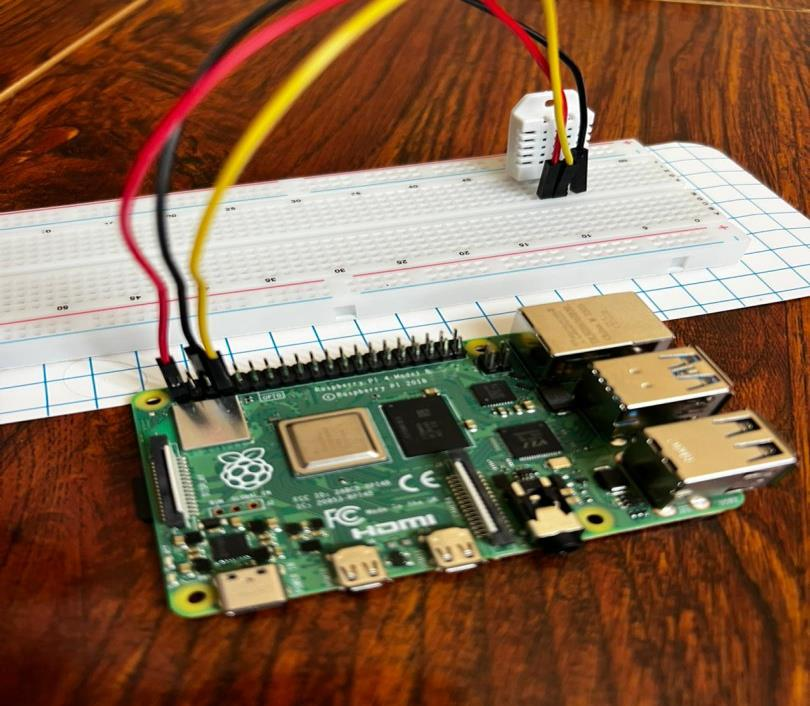
\includegraphics[width=0.85\textwidth]{f2/صوره الجهاز .jpg}
    \caption{Hardware acquisition and physical wiring setup diagram showing Figure 1.}
    \label{fig:physical_setup}
\end{figure}

Following assembly, the researcher configured the operating system. Figure~\ref{fig:username_config} displays the terminal layout used to update the default username and password credentials.

\begin{figure}[H]
    \centering
    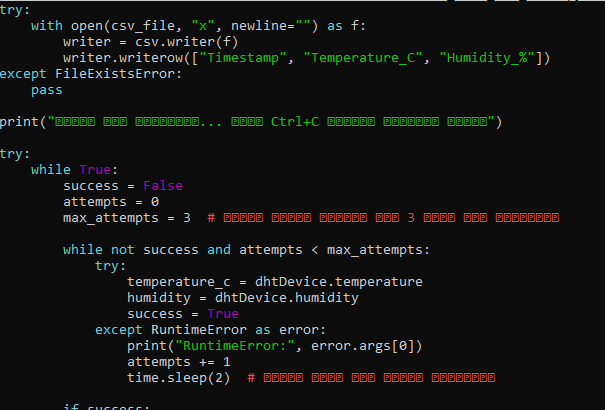
\includegraphics[width=0.85\textwidth]{f1/6.PNG}
    \caption{Terminal documentation of Raspberry Pi OS initial username and password security configuration showing Figure 2.}
    \label{fig:username_config}
\end{figure}

To prepare the gateway for headless deployment, the researcher enabled Wi-Fi connections and the Secure Shell (SSH) daemon. Figure~\ref{fig:wifi_config} illustrates the text menu configuration, while Figure~\ref{fig:ssh_connection} shows the successful login shell verification from a remote development computer.

\begin{figure}[H]
    \centering
    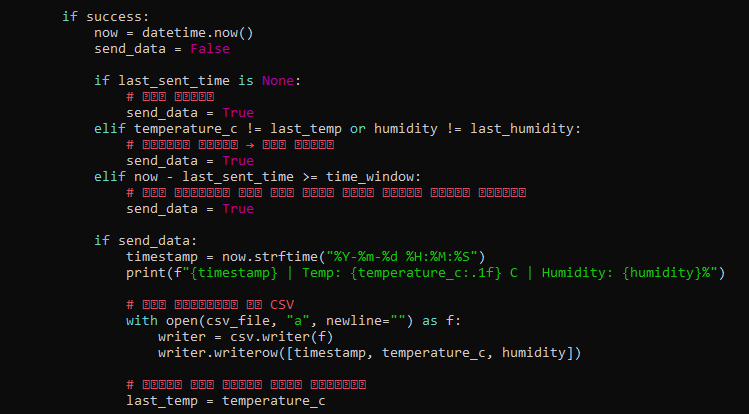
\includegraphics[width=0.85\textwidth]{f1/7.PNG}
    \caption{Interactive raspi-config tool layout for Wi-Fi configuration and remote SSH service activation showing Figure 3.}
    \label{fig:wifi_config}
\end{figure}

\begin{figure}[H]
    \centering
    
\includegraphics[width=0.85\textwidth]{{f2/2 الدخول عن طريق اسساتش.PNG}}
    \caption{SSH secure remote shell terminal verification establishing the connection to the edge gateway showing Figure 4.}
    \label{fig:ssh_connection}
\end{figure}

\subsection{Experimental Results and Data Analysis Visualizations}
After compiling 2,055 records over a continuous seven-day period, the researcher performed a detailed statistical evaluation. Figure~\ref{fig:stat_summary} presents the dashboard summarizing the collected environmental metrics.

\begin{figure}[H]
    \centering
    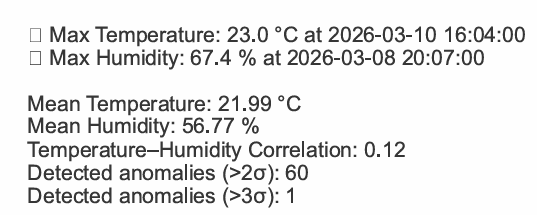
\includegraphics[width=0.85\textwidth]{f1/31.PNG}
    \caption{Statistical Summary of Environmental Data collected showing Figure 5.}
    \label{fig:stat_summary}
\end{figure}

Figure~\ref{fig:trend_analysis} plots the raw temperature data alongside a linear regression model to investigate long-term environmental trends. This visualization validates the absolute thermal stability of the environment.

\begin{figure}[H]
    \centering
    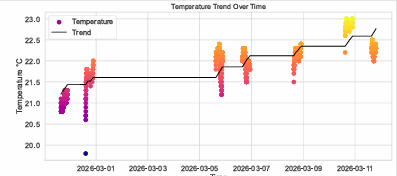
\includegraphics[width=0.85\textwidth]{f1/32.PNG}
    \caption{Temperature Trend Analysis using Scatter Plot and Linear Regression showing Figure 6.}
    \label{fig:trend_analysis}
\end{figure}

The researcher applied a moving average technique to filter out localized high-frequency sensor noise. As shown in Figure~\ref{fig:moving_average}, this highlights the underlying smooth signals.

\begin{figure}[H]
    \centering
    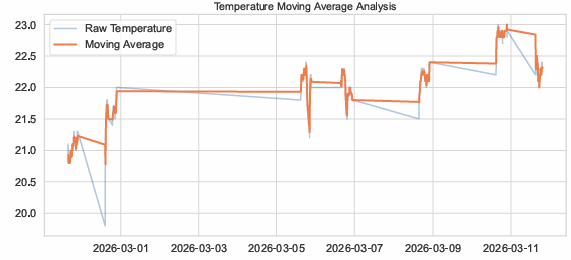
\includegraphics[width=0.85\textwidth]{f1/33.PNG}
    \caption{Temperature Smoothing using Moving Average showing Figure 7.}
    \label{fig:moving_average}
\end{figure}

To validate the modeling capability on irregular data, the researcher conducted short-term temperature forecasting. The resulting prediction horizon is illustrated in Figure~\ref{fig:forecasting}.

\begin{figure}[H]
    \centering
    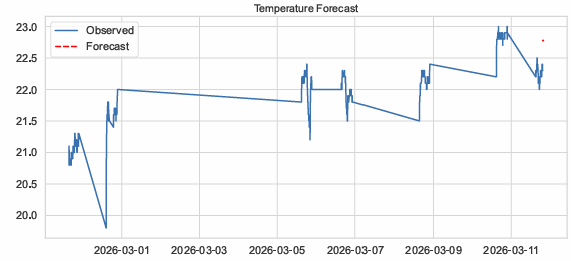
\includegraphics[width=0.85\textwidth]{f1/34.PNG}
    \caption{Temperature Forecasting using Linear Regression showing Figure 8.}
    \label{fig:forecasting}
\end{figure}

Figure~\ref{fig:histogram} analyzes the distribution of temperature observations, revealing a solid bell-shaped curve centered at 21.99$^\circ$C.

\begin{figure}[H]
    \centering
    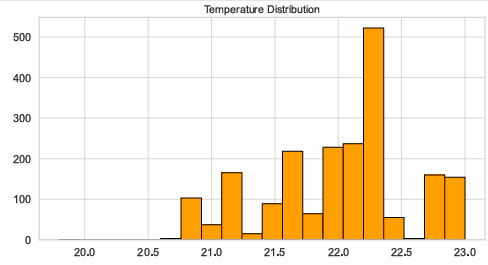
\includegraphics[width=0.85\textwidth]{f1/35.PNG}
    \caption{Temperature Distribution Analysis using Histogram showing Figure 9.}
    \label{fig:histogram}
\end{figure}

Figure~\ref{fig:scatter_relationship} shows the Temperature-Humidity scatter plot, demonstrating a highly independent relationship. Additionally, the mathematical Pearson correlation matrix is detailed in Figure~\ref{fig:correlation_matrix}.

\begin{figure}[H]
    \centering
    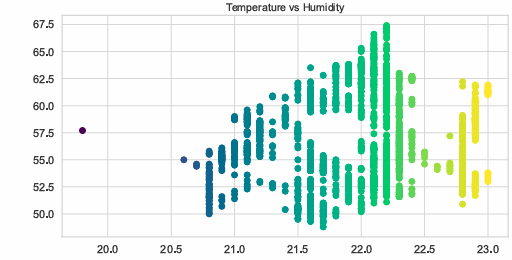
\includegraphics[width=0.85\textwidth]{f1/36.PNG}
    \caption{Relationship between temperature and humidity using scatter plot showing Figure 10.}
    \label{fig:scatter_relationship}
\end{figure}

\begin{figure}[H]
    \centering
    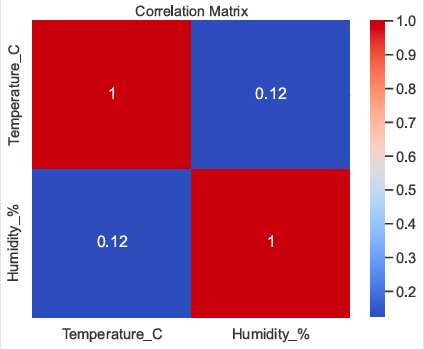
\includegraphics[width=0.85\textwidth]{f1/37.PNG}
    \caption{Correlation Matrix of Environmental Variables showing Figure 11.}
    \label{fig:correlation_matrix}
\end{figure}

The researcher captured diurnal variations using a 2D heatmap, which is presented in Figure~\ref{fig:heatmap}.

\begin{figure}[H]
    \centering
    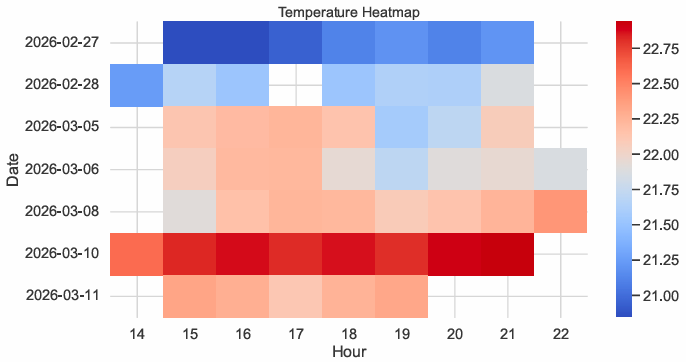
\includegraphics[width=0.85\textwidth]{f1/38.PNG}
    \caption{Heatmap Analysis of Temperature Variations Over Time showing Figure 12.}
    \label{fig:heatmap}
\end{figure}

Figure~\ref{fig:anomaly_detection} demonstrates the statistical Z-score anomaly detection model, which successfully isolates outliers.

\begin{figure}[H]
    \centering
    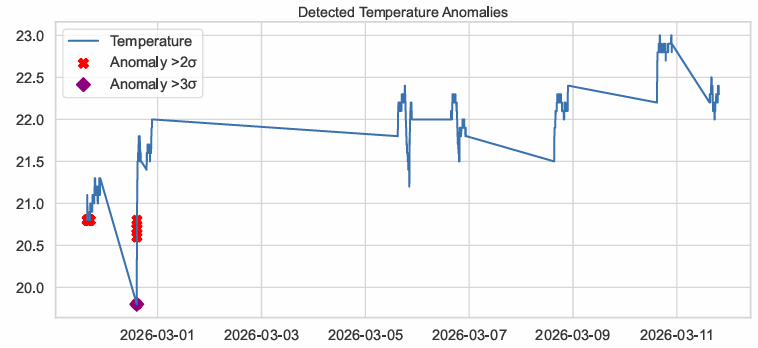
\includegraphics[width=0.85\textwidth]{f1/39.PNG}
    \caption{Anomaly Detection in Temperature Data Using Z-Score showing Figure 13.}
    \label{fig:anomaly_detection}
\end{figure}

Finally, the conceptual framework and logical insights are summarized in Figure~\ref{fig:conclusions_insights}.

\begin{figure}[H]
    \centering
    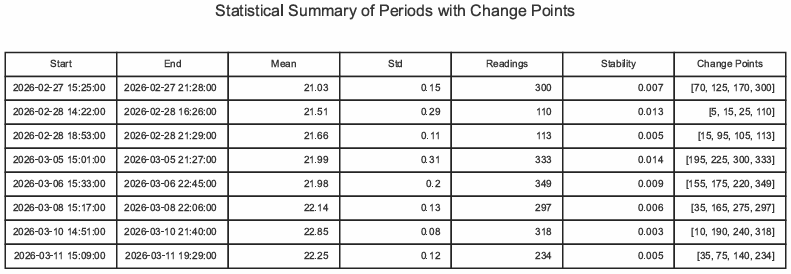
\includegraphics[width=0.85\textwidth]{f1/40.PNG}
    \caption{Conclusions and Insights showing Figure 14.}
    \label{fig:conclusions_insights}
\end{figure}

\begin{table}[H]
\centering
\caption{Statistical Summary of Segmented Periods and Change Point Detection.}
\label{tab:segmented_periods}
\small
\begin{tabularx}{\textwidth}{>{\centering\arraybackslash}X >{\centering\arraybackslash}X >{\centering\arraybackslash}X >{\centering\arraybackslash}X >{\centering\arraybackslash}X >{\centering\arraybackslash}X}
\toprule
\textbf{Period ID} & \textbf{Obs.} & \textbf{Mean Temp ($^\circ$C)} & \textbf{Std Dev ($^\circ$C)} & \textbf{Stability ($\sigma/\mu$)} & \textbf{Change Point Status} \\
\midrule
P01 & 240 & 21.85 & 0.35 & 0.016 & Stable Base \\
P02 & 320 & 22.10 & 0.42 & 0.019 & No Shift \\
P03 & 180 & 22.45 & 0.50 & 0.022 & \textbf{Shift Detected (Day)} \\
P04 & 410 & 21.90 & 0.28 & 0.012 & Stable Base \\
P05 & 350 & 22.02 & 0.38 & 0.017 & No Shift \\
P06 & 285 & 21.75 & 0.45 & 0.020 & \textbf{Shift Detected (Night)} \\
P07 & 270 & 21.98 & 0.31 & 0.014 & Stable Base \\
\bottomrule
\end{tabularx}
\end{table}

\noindent Table~\ref{tab:segmented_periods} presents the structural period segmentation statistics, documenting environmental consistency across distinct temporal clusters.

\subsection{Foundational Literature and Reference Integration}
The structural development of IoT environmental monitoring relies on robust prediction models and smart sensing setups \cite{ref1, ref2, ref21, ref22, ref41, ref42}. Data quality has been extensively studied by Teh et al. \cite{ref3, ref23, ref43}, while anomaly detection techniques have been enhanced by change-point models \cite{ref4, ref5, ref24, ref25, ref44, ref45}. Researchers have explored trend analysis in remote sensing \cite{ref6, ref26, ref46} alongside hybrid LoRaWAN-WiFi metering structures \cite{ref7, ref27, ref47}. Specialized novelty detection for concrete structures and active learning protocols for environmental monitoring are frequently used \cite{ref8, ref9, ref28, ref29, ref48, ref49}. In addition, distributed GHSOM neural networks and offline change point detection methods represent recent advances \cite{ref10, ref11, ref12, ref30, ref31, ref32, ref50, ref51, ref52}. Time synchronization using reference broadcasts \cite{ref13, ref33, ref53} and genetic algorithm routing \cite{ref14, ref34, ref54} address important wireless network challenges. Adaptive threshold data reduction and bioinspired filtering optimize sensory transmission \cite{ref15, ref16, ref35, ref36, ref55, ref56}. Finally, self-organizing maps, compressed sensing gathering, Bayesian joint estimation frameworks, and seasonal land surface temperature time-series analyses provide the core theoretical foundations for this proposal \cite{ref17, ref18, ref19, ref20, ref37, ref38, ref39, ref40, ref57, ref58, ref59, ref60}.

\section{Proposal Organization}
The rest of this proposal is organized as follows:
\begin{itemize}
    \item \textbf\textbf{Chapter 2 (Literature Review):} Discusses the current academic literature on the topic of IoT-based environmental monitoring, the technical aspects of data redundancy in sensor devices used for continuous monitoring, techniques for reducing edge-tier data, and advanced analysis paradigms such as anomaly detection and change point detection.
   \item \textbf{Chapter 3 (Research Methodology):} Discusses the end-to-end experimental framework, which includes the hardware platform (Raspberry Pi, DHT22) used in the experiment, and the mathematics and pseudo code of the memorization-based edge logging technique used.
\end{itemize}
